\begin{figure*}[t!]
    \definecolor{myred}{HTML}{FF0080}
    \definecolor{myblue}{HTML}{007FFF}
    \centering

    \tabcolsep=0.10cm
    \renewcommand{\arraystretch}{0.1}
    \setlength{\medmuskip}{-1mu}
    \begin{tabular}{cc}
        \raisebox{0.025\height}{
        \includegraphics[width=0.250\linewidth]{img/cubes/LF.pdf}
        }
        &
        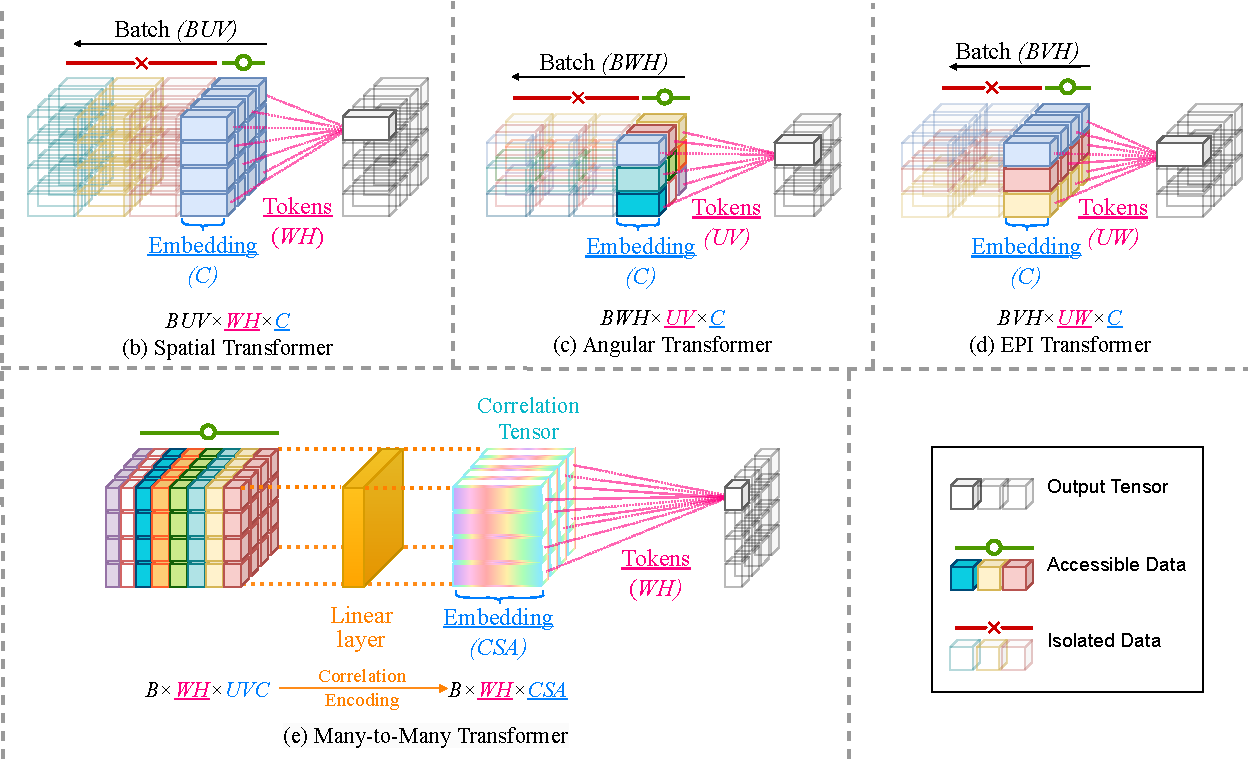
\includegraphics[width=0.660\linewidth]{img/cubes/main.pdf}
        % \begin{tabular}{ccc}
        %     \includegraphics[height=0.155\linewidth]{img/cubes/Spatial.pdf} &
        %     \includegraphics[height=0.155\linewidth]{img/cubes/Angular.pdf} &
        %     \includegraphics[height=0.155\linewidth]{img/cubes/EPI.pdf} \\
        %     \footnotesize $BU\!V \times \textcolor{myred}{\underline{W\!H}} \times \textcolor{myblue}{\underline{C}}$ &
        %     \footnotesize $BW\!H \times \textcolor{myred}{\underline{U\!V}} \times \textcolor{myblue}{\underline{C}}$ &
        %     \footnotesize $BV\!H \times \textcolor{myred}{\underline{U\!W}} \times \textcolor{myblue}{\underline{C}}$ \\
        %     \footnotesize (b) Spatial Transformer. &
        %     \footnotesize (c) Angular Transformer. &
        %     \footnotesize (d) EPI Transformer. \\
        %     \vspace{0pt} & \\
        %     \multicolumn{3}{c}{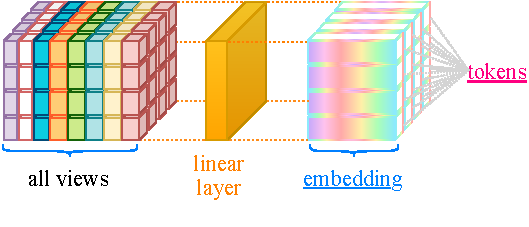
\includegraphics[height=0.18\linewidth]{img/cubes/SAT.pdf}} \vspace{-8pt} \\
        %     \multicolumn{3}{c}{\footnotesize $B \times \textcolor{myred}{\underline{W\!H}} \times \textcolor{myblue}{\underline{C_{SA}}}$} \\
        %     \multicolumn{3}{c}{\footnotesize (e) Spatial-angular Transformer.} \\
        % \end{tabular}
    \end{tabular}

    % \tabcolsep=0.20cm
    % \renewcommand{\arraystretch}{1}
    % \setlength{\medmuskip}{-1mu}
    % \begin{tabular}{ccccc}
    %     \includegraphics[width=0.1\linewidth]{img/cubes/LF.pdf} &
    %     \includegraphics[width=0.2\linewidth]{img/cubes/Spatial.pdf} &
    %     \includegraphics[width=0.2\linewidth]{img/cubes/Angular.pdf} &
    %     \includegraphics[width=0.2\linewidth]{img/cubes/EPI.pdf} &
    %     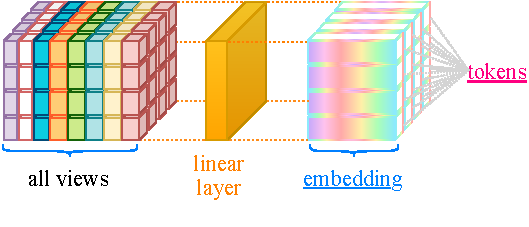
\includegraphics[width=0.2\linewidth]{img/cubes/SAT.pdf} \\
    %     \makecell{
    %         \footnotesize $U \times V \times W \times H \times C$ \\
    %         \footnotesize (a) LF image and tensor.
    %     } &
    %     \makecell{
    %         \footnotesize $U\!V \times \textcolor{myred}{\underline{W\!H}} \times \textcolor{myblue}{\underline{C}}$ \\
    %         \footnotesize (b) Spatial transformer. \\
    %     } &
    %     \makecell{
    %         \footnotesize $W\!H \times \textcolor{myred}{\underline{U\!V}} \times \textcolor{myblue}{\underline{C}}$ \\
    %         \footnotesize (c) Angular transformer. \\
    %     } &
    %     \makecell{
    %         \footnotesize $V\!H \times \textcolor{myred}{\underline{U\!W}} \times \textcolor{myblue}{\underline{C}}$ \\
    %         \footnotesize (d) EPI transformer. \\
    %     } &
    %     \makecell{
    %         \footnotesize $V\!H \times \textcolor{myred}{\underline{U\!W}} \times \textcolor{myblue}{\underline{C}}$ \\
    %         \footnotesize (e) Spatial-angular transformer. \\
    %     }
    % \end{tabular}
    \caption{Illustration of available data in LF tensors used by existing LF Transformers under the One-to-One scheme and our proposed Many-to-Many Transformer. For the tensors, each color represents a SAI.}
    \label{fig:Cubes}
\end{figure*}
